\documentclass[12pt]{article}

% margins and page style
\usepackage[margin=2.5cm]{geometry}
\usepackage{fancyhdr}
\pagestyle{fancy} 

% spaces between paragraphs
\usepackage[parfill]{parskip}

% fonts
\usepackage[T1]{fontenc}
\usepackage[scaled=0.92]{helvet}
\renewcommand*\familydefault{\sfdefault}

% font size of section headings
\usepackage{sectsty}
\sectionfont{\fontsize{14}{15}\selectfont}

% tables 
\usepackage{booktabs}
\renewcommand{\arraystretch}{1.5}

% figures
\usepackage{graphicx}
\usepackage[font=small,labelfont=bf]{caption} 

% colors
\usepackage[dvipsnames,svgnames,hyperref,table]{xcolor}

% hyperlinks
\usepackage{hyperref}
\hypersetup{
  pdfauthor={Erin C. McKiernan},
  colorlinks=true,
  urlcolor=Bittersweet,
  linkcolor=blue,
  citecolor=Purple,
}

% bib options
\let\oldbibliography\thebibliography
\renewcommand{\thebibliography}[1]{\oldbibliography{#1}
\setlength{\itemsep}{0pt}} 
\usepackage[numbers,sort&compress]{natbib} 
\bibliographystyle{unsrtnat}

% title and authors
\title{\vspace{-1.8cm}\Large{\textbf{Investigating movements of the eye using electrooculography}}}
\author{}
%\author[1, \email]{Erin C. McKiernan} 

%\affil[1]{\small{Departamento de F\'isica, Facultad de Ciencias, Universidad Nacional Aut\'onoma de M\'exico}}

%\affil[ \email]{\small{emckiernan@ciencias.unam.mx}}
\date{}

%%%%%%%%%%%%%%%%%%%%%%%%%%%%%%%%%%%%%%%%%%%%%%%%%%%%%%%%%%%%
 
\begin{document}
\maketitle

\vspace{-1.4cm}

\section*{OVERVIEW}

In this laboratory practical, students will record movements of the eye using electrooculography. In addition, students will explore how the electrical signals change, if at all, under different light conditions. Overall, this practical will help students understand the control of eye movements and the generation of electrical signals in the eye.

\section*{SPECIFICATIONS}
\begin{tabular}{p{6cm} p{10cm}}
\textbf{Level of study:} & Undergraduate \\
\textbf{Degree programs:} & Biology, Physics, Biomedical Physics, others \\
\textbf{Semester:} & 4th to 6th (i.e. 2nd to 3rd year undergrads) \\ 
\textbf{For use in courses:} & Systems Physiology, Physics of the Human Body, others \\
\textbf{Recommended prior courses:} & Molecular \& Cellular Biology \\
\textbf{Duration of practical:} & 1 hour \\
\textbf{Setting:} & Classroom or laboratory \\
\textbf{Safety considerations:} & skin around the eyes is sensitive; take care and remove surface electrodes slowly to avoid injury \\
\end{tabular}

\section*{OBJECTIVES}
\textbf{Before doing this lab you should be able to:}
\begin{itemize}
\item describe the basic structure of the eye
\item identify and locate the primary ocular muscles
\item understand electric dipoles and potentials 
\end{itemize}
 
\vspace{0.3cm}

\textbf{In this lab you will:}
\begin{itemize}
\item learn how to record an electrooculogram (EOG) 
\item observe and record EOG deflections when eyes move up and down or side to side
\item observe and record how the standing potential of the eye varies in different light conditions 
\end{itemize}

\vspace{0.3cm}
 
\textbf{After doing this lab you should be able to:}
\begin{itemize}
\item understand how electrical signals in the eye are generated
\item understand how these signals change in response to movement and light
\item explain the differences and relationship between EOG and EMG recordings
\item design further experiments to study eye movements and responses to light
\end{itemize}

\section*{EQUIPMENT}

\begin{itemize}
	\item Heart \& Brain SpikerShield with integrated Arduino (Backyard Brains)
   	\item 3 surface electrodes (Backyard Brains or other provider)
    \item cable with alligator clips to connect electrodes to SpikerShield (Backyard Brains)
    \item USB cable to connect SpikerShield to computer (Backyard Brains)
    \item computer with free Backyard Brains SpikeRecorder software installed (note that a smartphone or tablet will not work, since cable connects to USB port)
\end{itemize}

\section*{BACKGROUND}

\subsection*{Types of eye movement}

Eye movements are a necessary part of functional vision, allowing us to adjust for head position, change the focus of our attention, track objects, and much more \cite{foulsham2015eye,schor2011neural}. We can classify eye movements in several different ways depending on the factor of interest. Movements can be either voluntary (e.g., purposefully directing gaze towards a particular object), or involuntary/reflexive (e.g. rapid eye movements that occur during sleep). Movements can also be either conjugate (both eyes move in the same direction), or disjunctive (the eyes move in different directions) \cite{mather2016foundations}. In this practical, we will ask subjects to move both eyes from one side to another, or up and down. Therefore, we will be investigating voluntary, conjugate eye movements. To be more specific, we will study voluntary saccades, which are quick movements of the eyes as they shift from one fixation point to the next \cite{mather2016foundations}.

The eyes can move in different directions and each of these movements has a special name. Movement of the eye toward the midline is called adduction, while movement in the opposite direction, laterally, is called abduction \cite{purves2001editors}. Upward movement of the eye is elevation, while downward movement is depression. Finally, medial rotation is known as 
intorsion, while lateral rotation is extorsion. These movements are each controlled by one to two extraocular muscles \cite{purves2001editors}.

\subsection*{Extraocular muscles}

There are 6 extraocular muscles which contract to move the eye in different directions (Fig. \ref{fig:eyeMuscles}) \cite{openStax2017sensory}. These muscles are:

\vspace{0.3cm}

\begin{itemize}
\item \textbf{medial rectus}: contraction pulls eye toward the midline, produces adduction
\item \textbf{lateral rectus}: contraction pulls eye away from the midline, produces abduction
\item \textbf{superior rectus}: contraction pulls eye upward, contributes to elevation
\item \textbf{inferior rectus}: contraction pulls eye downward, contributes to depression
\item \textbf{superior oblique}: contraction rotates eye medially (intorsion); also contributes to depression 
\item \textbf{inferior oblique}: contraction rotates eye laterally (extorsion); also contributes to elevation
\end{itemize}

\vspace{0.3cm}

Eye adduction and abduction typically require the contraction of only one muscle at a time, either the medial or lateral rectus, respectively \cite{purves2001editors}. Elevation and depression, in contrast, are slightly more complex than horizontal movements because the eye is not aligned such that the inferior and superior muscles pull straight up or down. They instead pull at slight angles, and their movement must be accompanied by compensatory pulling from the oblique muscles \cite{openStax2017sensory}. Thus, the superior rectus works with the inferior oblique to achieve elevation, while the inferior rectus and superior oblique together produce depression \cite{purves2001editors} (Fig. \ref{fig:eyeMuscles}). 

\begin{figure}[h!]
\centering
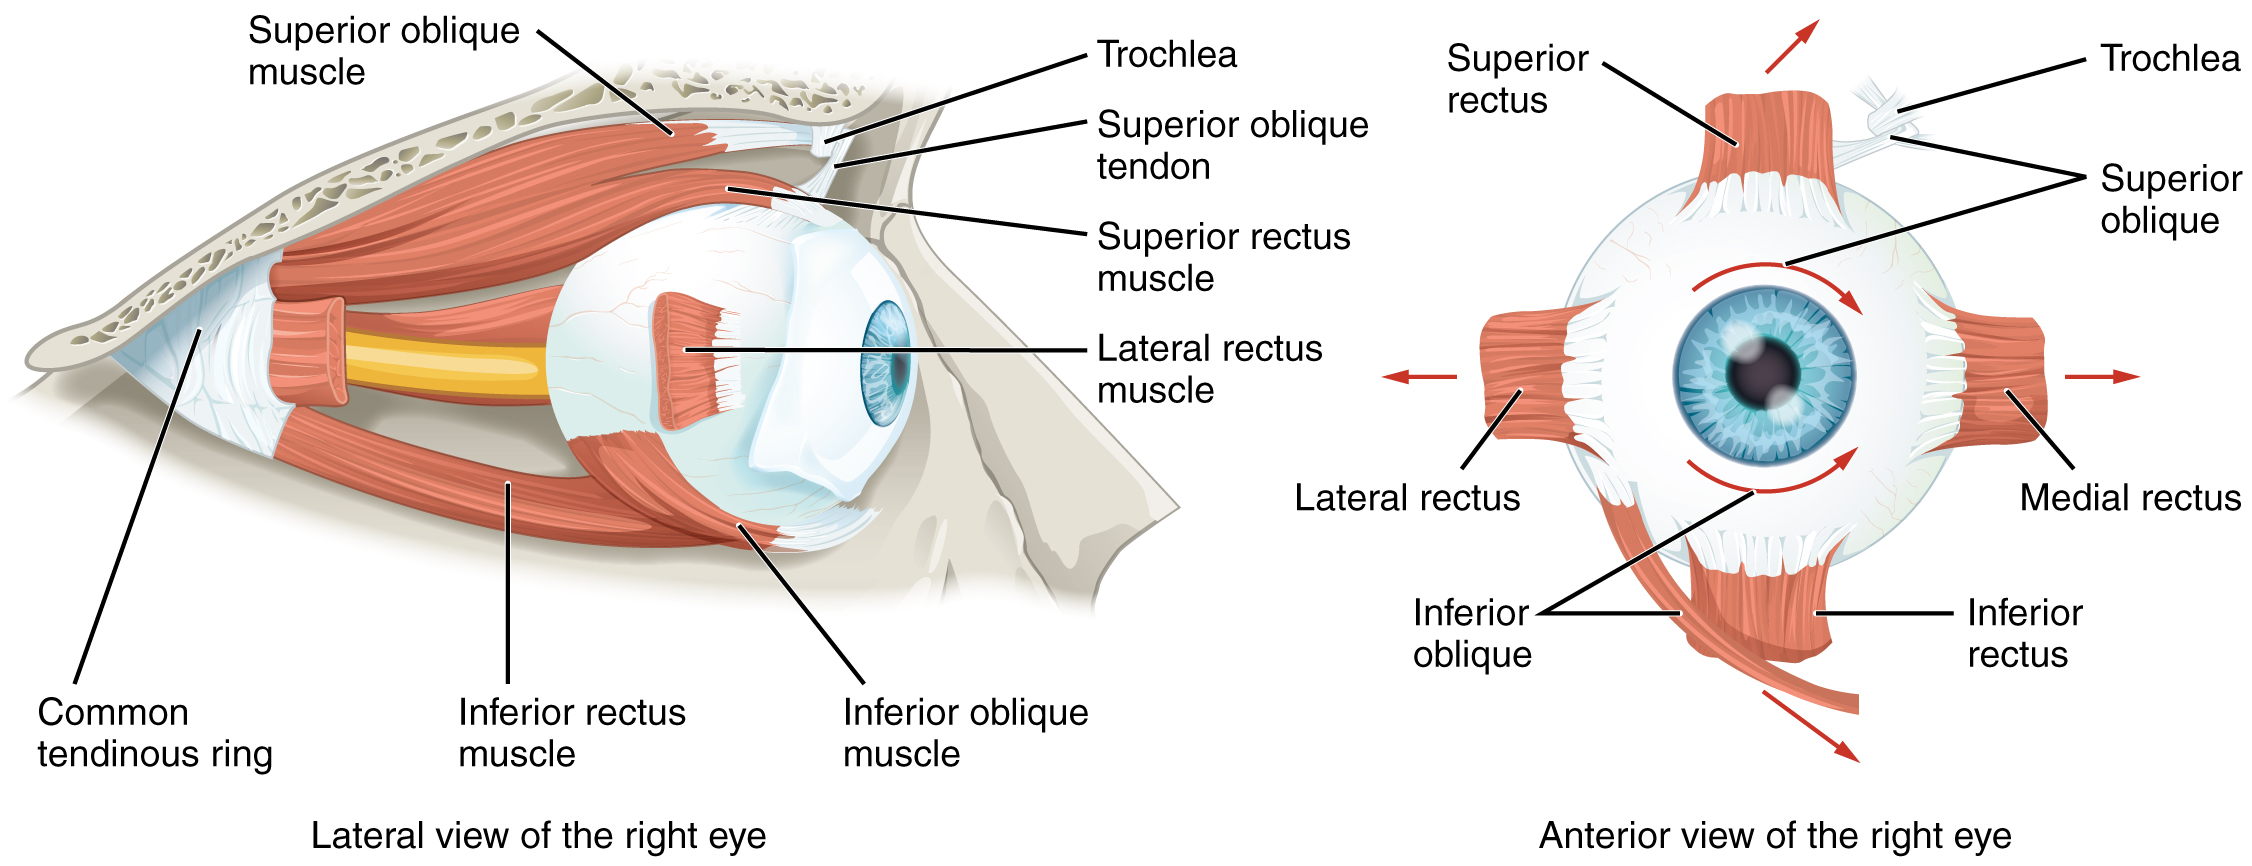
\includegraphics[width=0.95\textwidth]{images/extraocularMuscles.jpg}
\caption{Extraocular muscles. Image credit: OpenStax \cite{openStax2017sensory}, Creative Commons Attribution license (CC BY).}
\label{fig:eyeMuscles}
\end{figure}

\subsection*{Measuring eye movements produced by ocular muscles}

Ideally, we would like to record the activity of the extraocular muscles using electromyography (EMG). However, as we saw in the practical `Basics of Electromyography', non-invasive (surface electrode) recordings are difficult to obtain from some muscles, especially if the muscles are not located supeerficially but in deeper layers. Extraocular muscles are located 
within the eye socket and above them lie facial muscles such as the obicularis oculi, which control movements of the eyelids. Thus, it is likely that any surface EMG recording we attempted around the eye would pick up activity from these muscles, rather than our muscles of interest. Therefore, we will need to find another way to record eye movements. Fortunately, other electrical properties of the eye provide such an alternative. 

%While the extraocular muscles have the same striated structure and the same contraction mechanisms as typical skeletal muscle, there are important differences. For example, while many skeletal muscle motor units are silent at rest, motor units of the eye show high levels of baseline activity. This tonic firing is in the range of 100-150 Hz, and is so pronounced that some have said there is really ``no position of rest for extraocular muscles" \cite{breinin1955electromyography}. Thus, what we will be looking for as an indication of muscle activation associated with eye movement will not be the beginning of firing after a period of quiescence, as with a bicep or similar, but rather a dramatic increase in the firing rate. To overcome the viscous forces opposing saccadic-type movements in the eye, extraocular motor units will show bursts of rapid firing as high as 600 Hz. The firing rate decreases again when the eye reaches the new position.

\subsection*{Electric dipole}

An electric dipole is formed by two charges of opposite sign, $q^+$ and $q^-$, separated by a distance, $d$ \cite{hyperphysicsDipole}. The electric dipole moment is a vector, $\vec{p}$, given by the product of the charge magnitude, $q$, and the distance between the two charges. By convention, the vector points from the negative to the positive charge (Fig. \ref{fig:dipole}). 

\begin{figure}[h!]
\centering
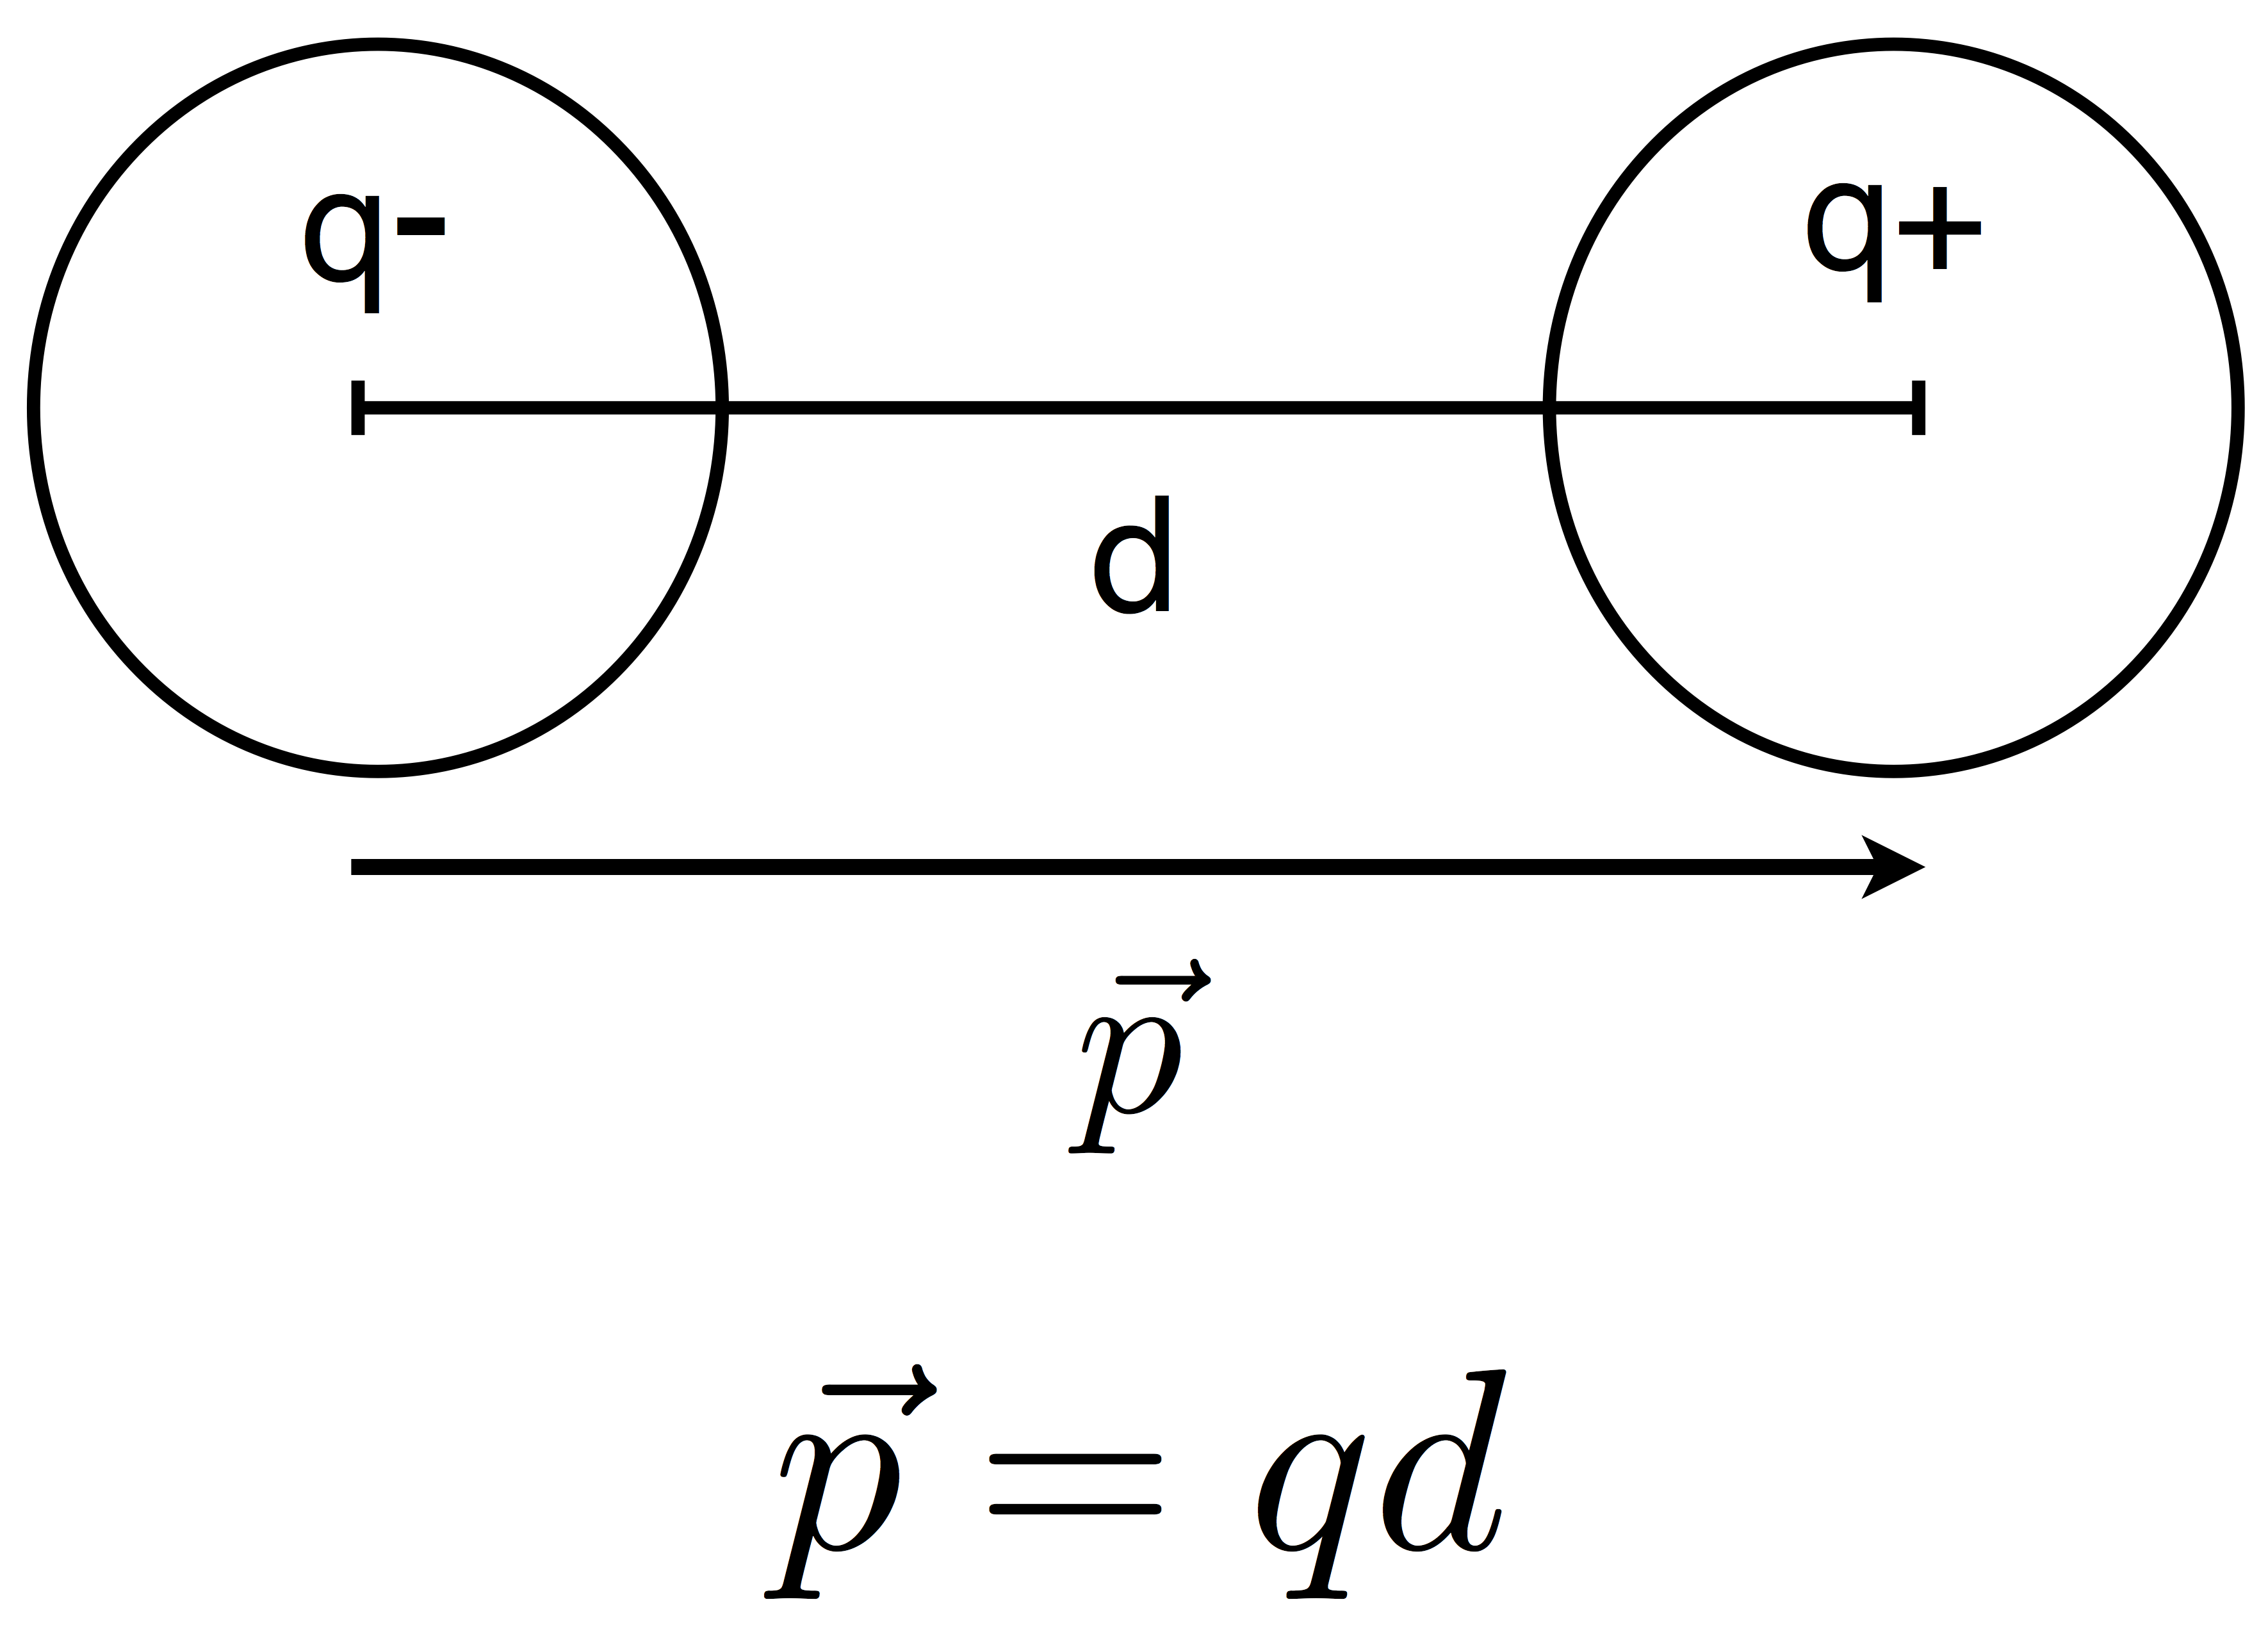
\includegraphics[width=0.5\textwidth]{images/dipole.png}
\caption{Schematic representation of an electric dipole. Image credit: Erin C. McKiernan, CC BY.}
\label{fig:dipole}
\end{figure}

\subsection*{Dipole of the eye}

There is a potential difference between the cornea and the retina, called the corneoretinal potential (CRP) or the standing potential of the eye \cite{heide1999electrooculography,marg1951development,malmivuo1995bioelectromagnetism}. The cornea is positive relative to the negative potential in the retina, thus establishing an electric dipole which points from the back to the front of the eye (Fig. \ref{fig:crp}). Movement of the eye will cause the dipole to move and change the surrounding electric field. As we will see, we can measure these changes with the electrooculogram.

\begin{figure}[h!]
\centering
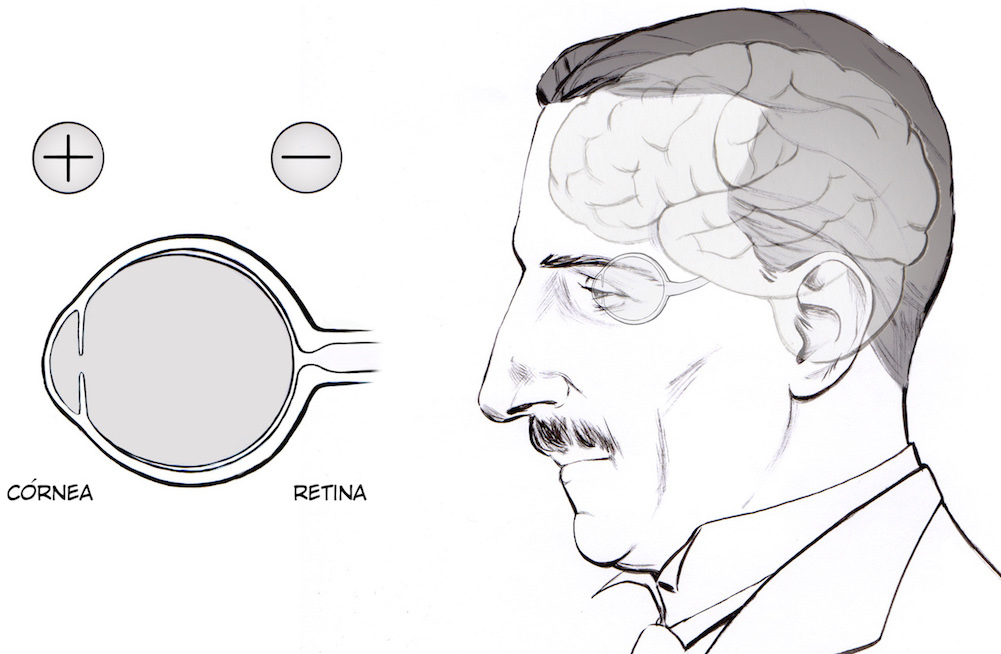
\includegraphics[width=0.7\textwidth]{images/eyePolarity.jpg}
\caption{The electric dipole of the eye. Image credit: Backyard Brains, CC BY-SA.}
\label{fig:crp}
\end{figure}

The standing potential of the eye is largely due to the potential difference across the retinal pigment epithelium (RPE) \cite{heide1999electrooculography,berg1991dipole}, the transepithelial potential (TEP). The TEP is established and maintained by the transport of ions across the apical and basolateral membranes of the epithelial cells \cite{joseph1991apical,quinn1992ion}. This transport is accomplished by specialized transmembrane proteins known as ion channels and pumps \cite{khanTransport}. Ion channels open to allow ions to flow in or out of the cell along their electrochemical gradients. Pumps come in a variety of types, including symporters that co-transport ion in the same direction and exchangers that bring one ion in while sending another ion out. Pumps may directly or indirectly use ATP to transport ions against their electrochemical gradients \cite{khanTransport}. 

Any change in the ion transport across the epithelial layer will alter the TEP and in turn be reflected in the CRP recorded via the electrooculogram (EOG). The amplitude of the CRP recorded in the EOG typically ranges from hundreds of microvolts ($\mu$ V) to one millivolt (mV). The TEP varies with light-dark conditions \cite{heide1999electrooculography}.

\subsection*{Electrooculogram}

Electrooculography measures changes in the electrical dipole of the eye and the recordings we obtain are called electrooculograms (EOGs) \cite{heide1999electrooculography,marg1951development,malmivuo1995bioelectromagnetism}. Similar to what we saw in the `Basics of Electromyography' practical, the EOG is a differential recording in which we place two electrodes, subtracting the signals recorded at the two points, and then amplify the difference. 
When the eyes are in the resting position, looking straight forward, the electrodes do not register any difference in potential. However, as the eyes move in a given direction, the positive end of the dipole moves closer to one electrode and farther away from the other. Since we are measuring the difference between the potentials recorded at the two electrodes, this will result in a positive deflection when the eyes move in one direction and a negative deflection when they move in the other direction \cite{malmivuo1995bioelectromagnetism} (Fig. \ref{fig:eog}).

\vspace{0.5cm}

\textbf{Study questions:}

\begin{itemize}
\item How will you place your electrodes to record elevation and depression of the eye?
\item How will you place your electrodes to record adduction and abduction of the eye?
\end{itemize} 

\begin{figure}[t!]
\centering
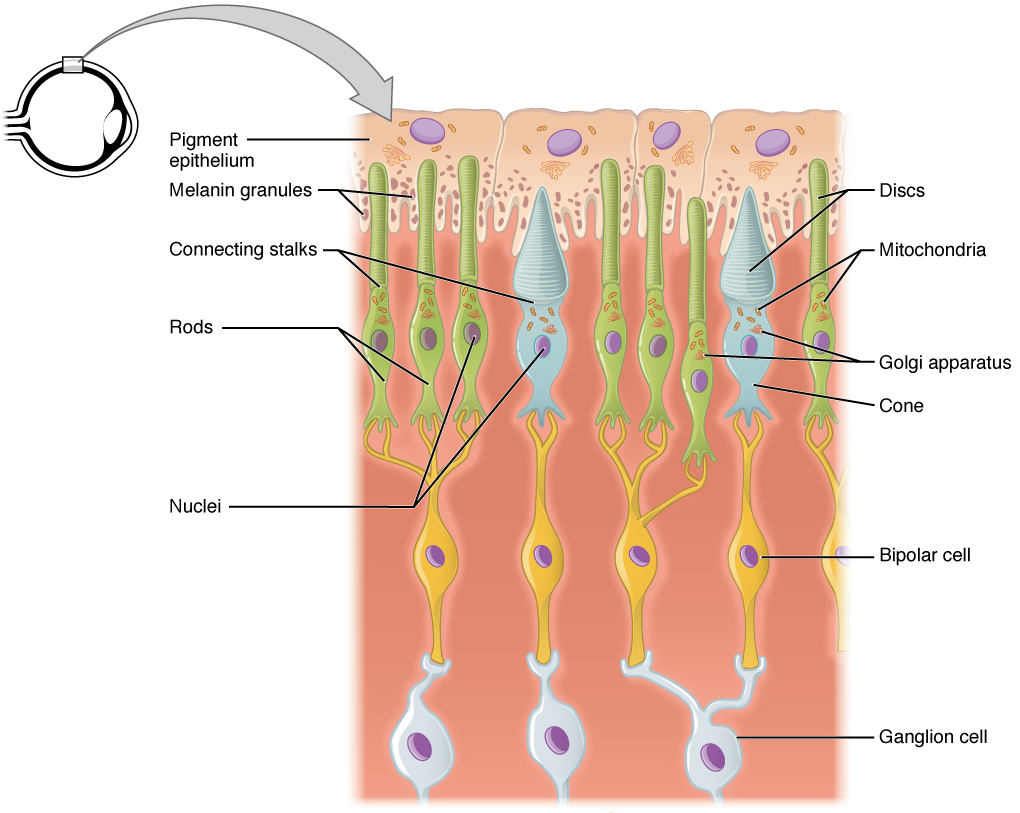
\includegraphics[width=0.81\textwidth]{images/rpe.png}
\caption{Organization of the eye showing the  retinal pigment epithelium (RPE). Image credit: OpenStax \cite{openStax2017sensory} }
\label{fig:rpe}
\end{figure}

\begin{figure}[b!]
\centering
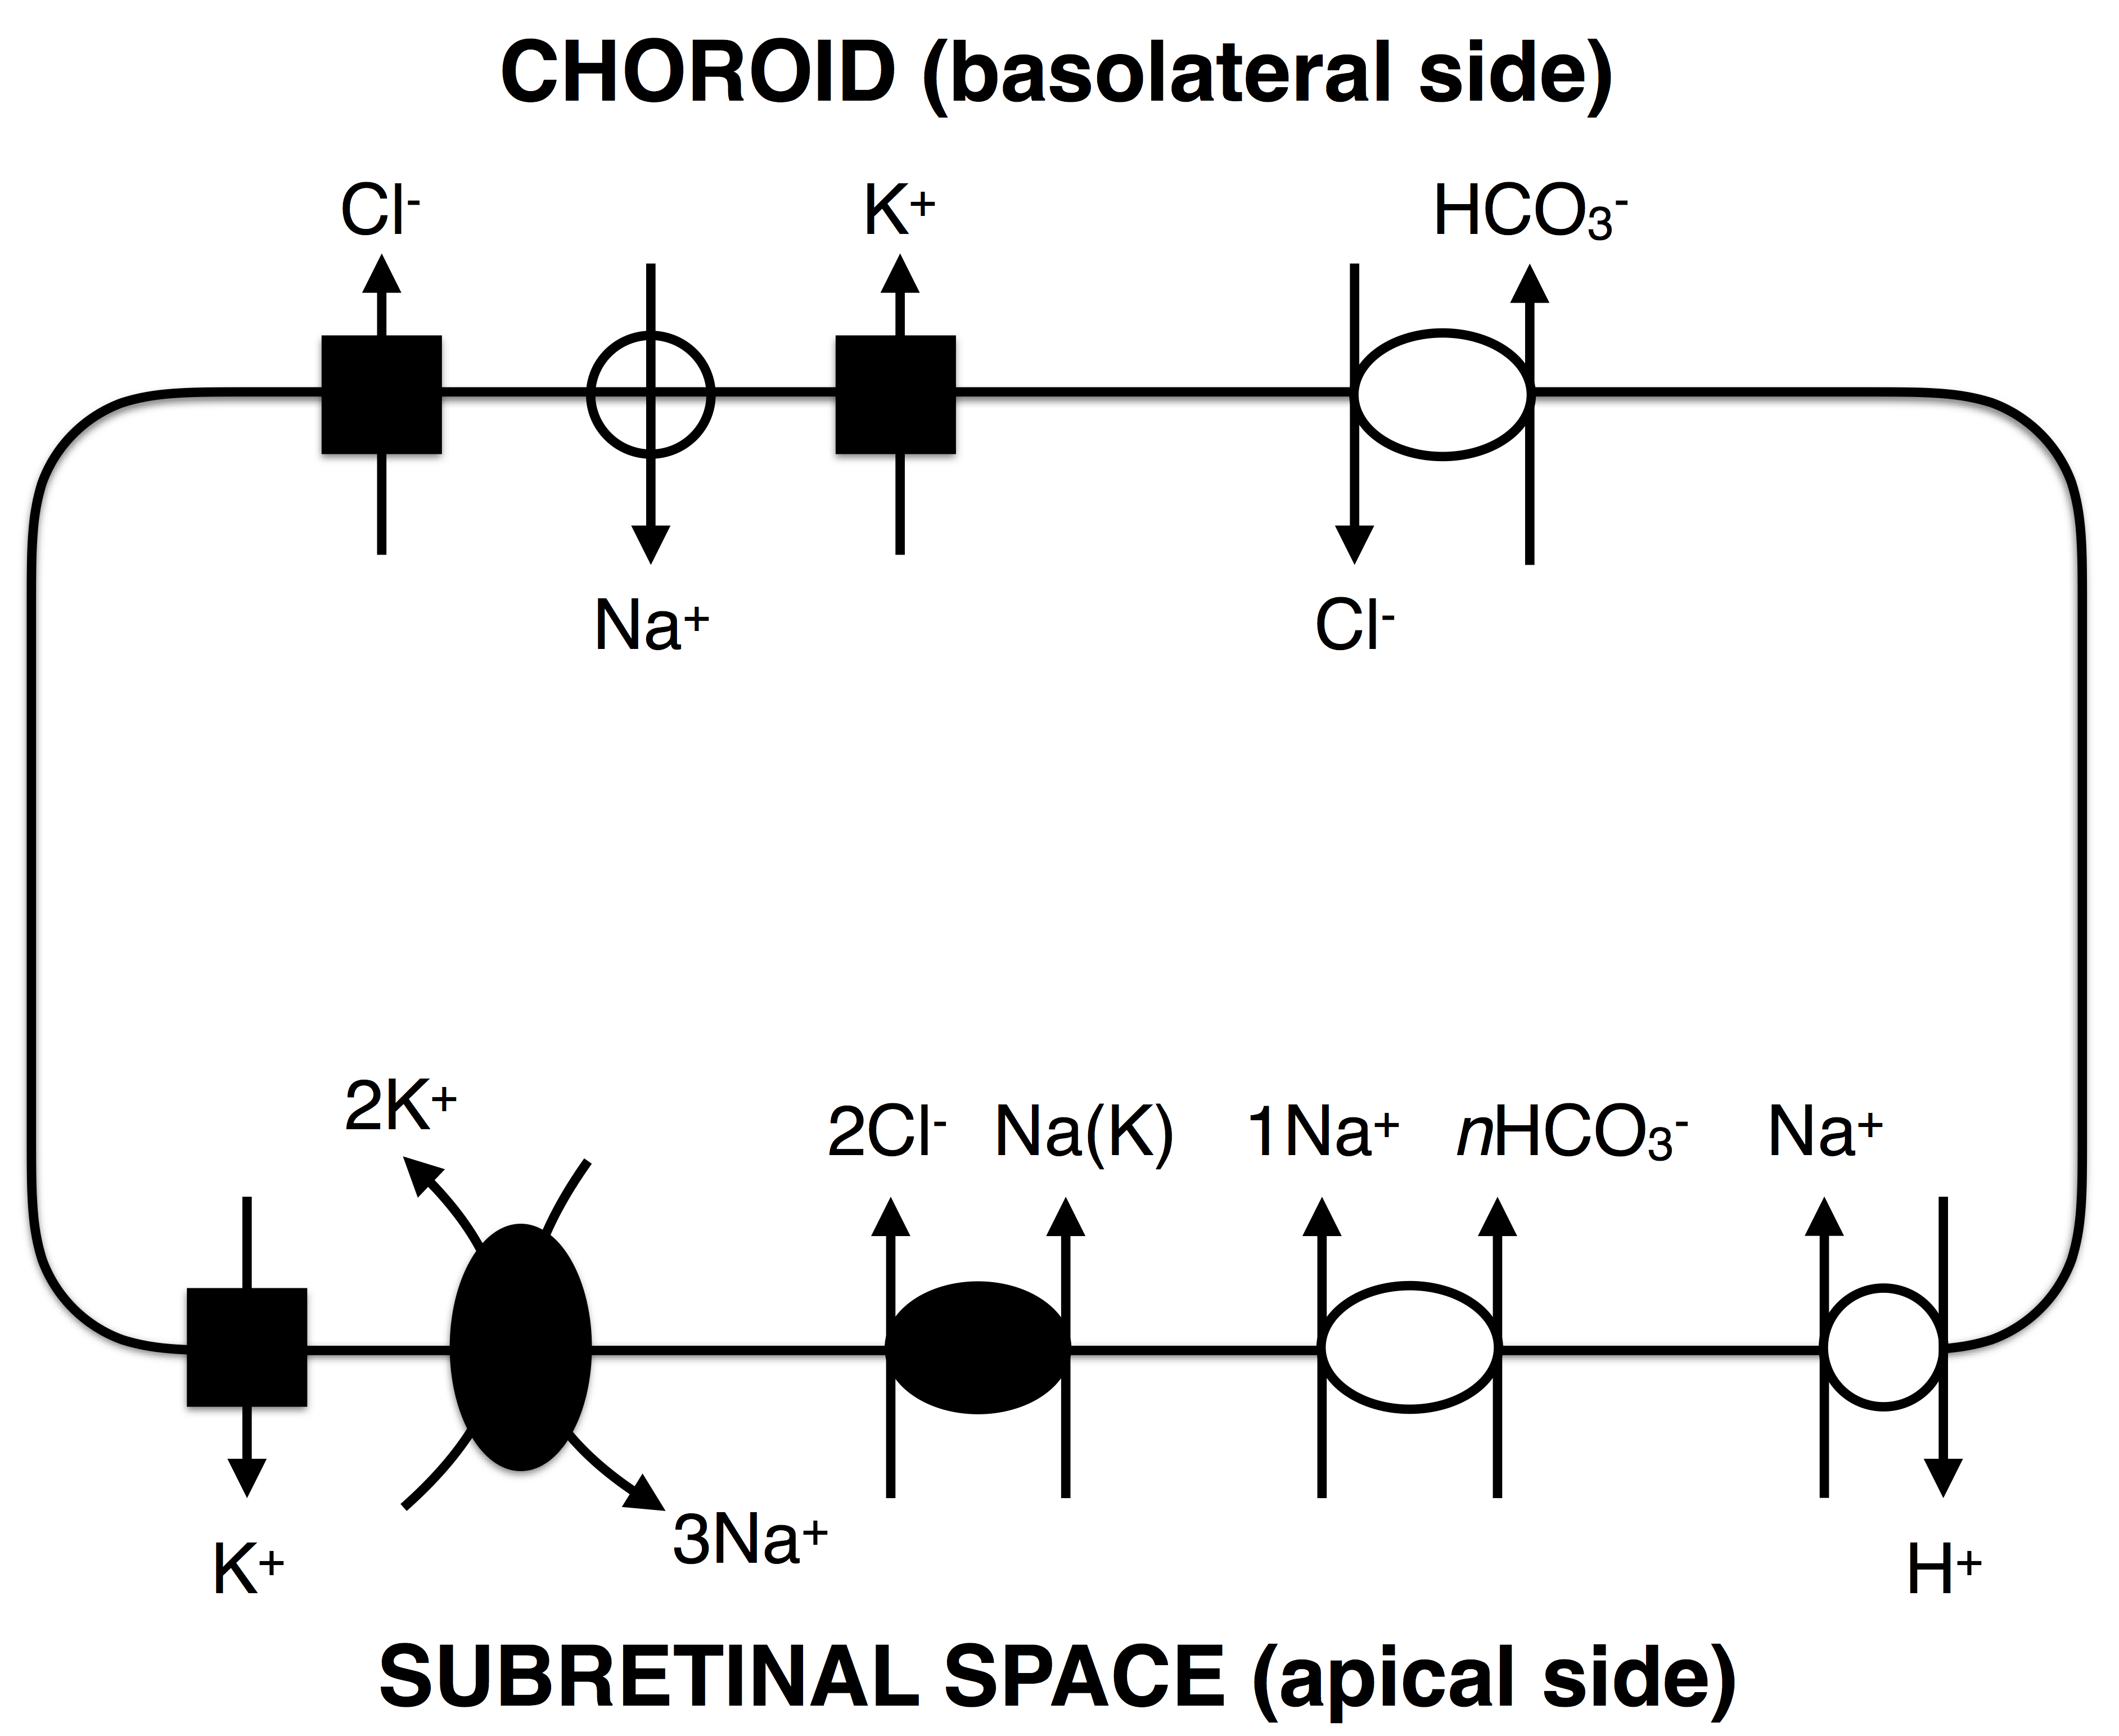
\includegraphics[width=0.63\textwidth]{images/rpeTransport.png}
\caption{Ion transport via channels and pumps in the RPE. Image credit: Erin C. McKiernan, CC BY. Based on information in \cite{joseph1991apical,quinn1992ion}}
\label{fig:crp}
\end{figure}

\begin{figure}[h!]
\centering
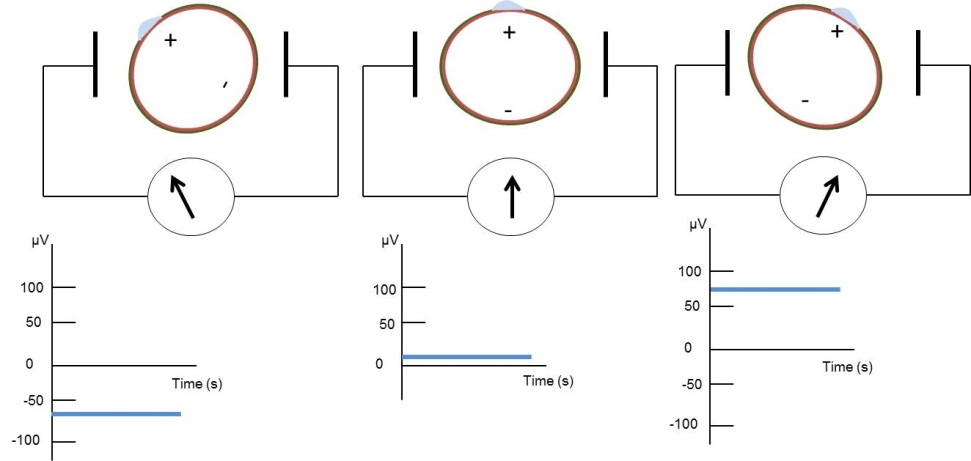
\includegraphics[width=0.95\textwidth]{images/eog.jpeg}
\caption{Schematic of an EOG recording. The top plots show the position of the eye and its dipole, while the bottom plots show the EOG singlas recording in microvolts. In the resting position (middle column), the electric dipole of the eye is oriented straight forward and little to no potential difference is recorded bteween the two electrodes. When the eyes move to the left (left column), the positive end of the dipole moves toward the left electrode and produces a negative deflection in the EOG. When the eyes move to the right (right column) the positive end of the dipole moves toward the right electrode and produces a positive deflection in the EOG. Image credit: \cite{viqueira2013ocular}}
\label{fig:eog}
\end{figure}

\section*{PROCEDURE}

Before beginning, make sure you have all the necessary equipment and have installed the recording software on your computer or smartphone. The Backyard Brains equipment comes assembled and ready to record. The following steps will guide you in assembling the equipment and carrying out recordings.

\subsection*{1. Setup EOG recordings}

\begin{enumerate}
\item Connect the 9V battery to its terminals on the Heart and Brain SpikerShield Box
\item Connect the blue USB cable to the Arduino port on the Heart and Brain SpikerShield Box
\item Connect the other end of the USB cable to your computer 
\item Connect the orange cable to its corresponding port on the Heart and Brain SpikerShield Box
\item Place the surface electrodes to first record eye elevation and depression, with one surface electrode above the eye and one below (Fig. \ref{fig:ePlacement}A,B). Afterwards, record adduction and abduction, with one surface electrode to the left of the left eye and one to the right of the right eye (Fig. \ref{fig:ePlacement}C)
\item The reference electrode should be placed behind one ear, just over the mastoid process (Fig. \ref{fig:ePlacement}A,D)

\vspace{0.2cm}

\begin{figure}[h!]
\centering
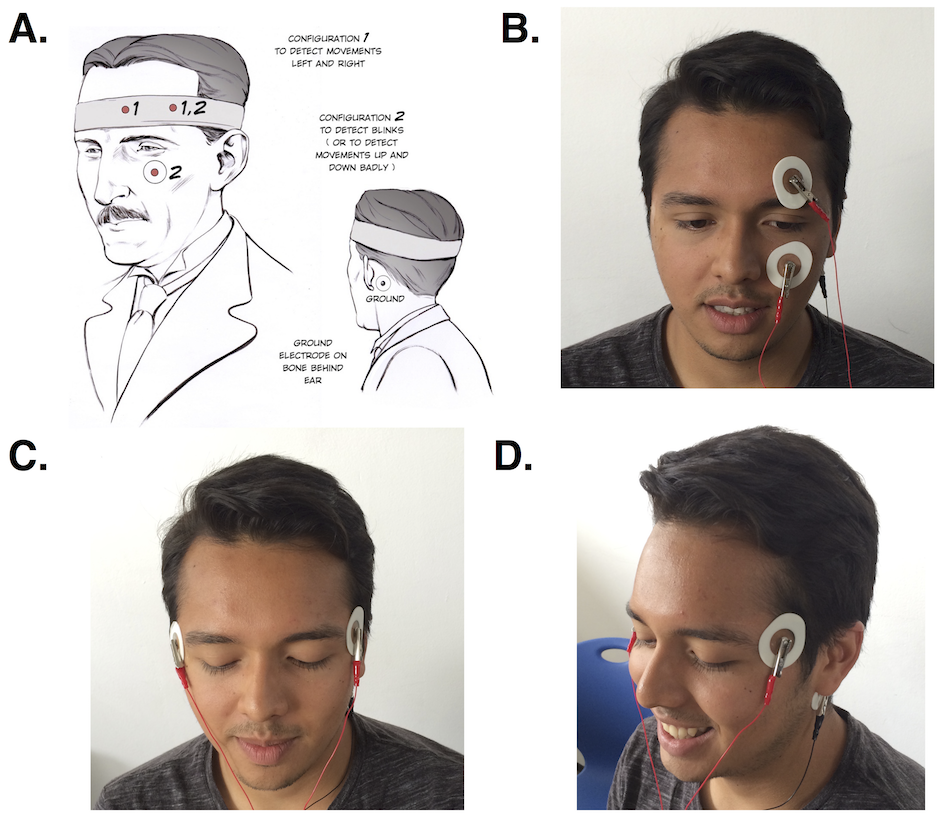
\includegraphics[width=0.9\textwidth]{images/eogElectrodes.png}
\caption{A. Cartoon showing two possible electrode placements. Image credit: Backyard Brains, CC BY-SA. B,C. Electrode placement to record elevation and depression (B.) or adduction and abduction (C). D. Placement of the reference electrode . Image credits B-D: Erin McKiernan, CC BY.}
\label{fig:ePlacement}
\end{figure}

\item Connect each of the red aligator clips on the end of the orange cable to one of the surface electrodes; make sure the metal clips do not touch and try to avoid entangling the cables
\item Connect the black aligator clip (reference) to the electrode placed behind the ear
\item To improve the EMG signal, the area where the electrodes will be placed can be cleaned with alcohol prior to placement; wait until the area is dry to place the electrodes
\item Electrode gel can be placed to improve conduction but is often not necessary
\item To avoid noise artifacts, ensure that no clothing is touching the electrodes or brushing against the cables during recording
\end{enumerate}

\subsection*{2. Test EOG recordings}

\begin{enumerate}
\item The Heart and Brain SpikerShield Box will turn on automatically when 
connected to the computer, indicated by the green light 
\item Open the Backyard Brains recording software and explore the controls and settings (for more info on software use, see [\cite{spikeRecorder}]) 
\item Ask the subject to briefly move their eyes and check that a corresponding deflection is seen in the recording
\item Try saving a test recording to your computer (format will be .wav)
\end{enumerate}

\subsection*{3. Collect your data}

\begin{enumerate}
\item Make sure the subject is in a resting position with eyes facing forward
\item When the subject is ready, press record on the Backyard Brains software interface
\item Instruct the subject to remain relaxed for 3-5 seconds after the recording begins, then move their eyes upward to record elevation
\item Next, ask the subject to return to the resting position for 3-5 seconds 
\item Then, instruct the subject to move their eyes downward to record eye depression
\item Ask the subject to repeat the above sequence 3 times 
\item Terminate the recording and save the data to your computer
\item Start a new recording to examine the effect of the size of the eye movement
\item To assist the subject in making eye movements of different magnitudes, place your finger at 3 different heights above or below the eye to serve as new fixation points
\item Terminate the recording and save the data to your computer 
\item EOG should be saved and exported in .wav format for analysis
\item Change the electrode placement to record adduction and abduction and repeat steps 1-11
\end{enumerate}

\section*{ACKNOWLEDGMENTS}
This work was supported by UNAM-DGAPA-PAPIME PE213817 and PE213219.

% BIBLIOGRAPHY
\renewcommand\refname{REFERENCES}
\renewcommand{\markboth}[2]{}%
\begin{footnotesize}
\bibliography{eye}
\end{footnotesize}

\end{document}
